\section{Method: Action Design Research - Drools in MPS}
\label{section:Method_action_research}

Even though Drools is a relatively small DSL, we did not need to implement all the functionality to answer our questions.
For this reason, we created smaller versions of the language.

\subsection{Really Simple Drools Language}
As we were new to DSL design and MPS, we first would create a simple approximation of the Drools language to create our first projections.
We called this language ``Really Simple Drools'' (RSD).

\paragraph{File} RSD, Like Drools itself, has a \texttt{File} as its root node.
The \texttt{File} only contains \texttt{Facts} and \texttt{Rules}.

\paragraph{\texttt{Fact} and \texttt{FactProperty}} In Drools, a \texttt{Fact} represents a Java Bean with its child properties, which can also have their child properties, ad infinitum.
In RSD, we limited properties to allow only boolean values.
We decided this because fact selection is a predicate and thus can only return a boolean.
By only allowing booleans, we also simplify the operations allowed on the property.

\paragraph{\texttt{Rule}} We only simulated the Left-hand side, or the ``\texttt{when}'' conditions, of a Drools Rule for the \texttt{Rule} Concept.
We believed this would provide us with compelling options for projections and did not want to overcomplicate this first approach.

An RSD Rule consists of a collection of conditions.
Should all those conditions return \texttt{true}, then the \texttt{Rule} is selected.

\paragraph{Condition} A condition operates on one or more \texttt{FactSelectors}.
There are four condition types \texttt{ExistsCondition}, \texttt{NotCondition}, \texttt{AndCondition}, and \texttt{OrCondition}.
\texttt{ExistsCondition} and \texttt{NotCondition} are unary conditions and evaluate one \texttt{FactSelector}.
\texttt{AndCondition} and \texttt{OrCondition} conditions evaluate two \texttt{FactSelectors}.

\paragraph{\texttt{FactSelector}} A \texttt{FactSelector} consists of a reference to a \texttt{Fact} and a collection of \texttt{Predicates}.
If the \texttt{Fact} exists and all the \texttt{Predicates} evaluate to \texttt{true}, then the \texttt{FactSelector} evaluates to \texttt{true}.

\paragraph{\texttt{Predicate}} The \texttt{Predicate} is an operation on a \texttt{FactProperty}, to which the Concept has a reference.
Because \texttt{FactProperty} represents a boolean value, the only predicate operations are ``\texttt{Is}'' and ``\texttt{Not}''.

\begin{figure}
    \centering
    \fbox{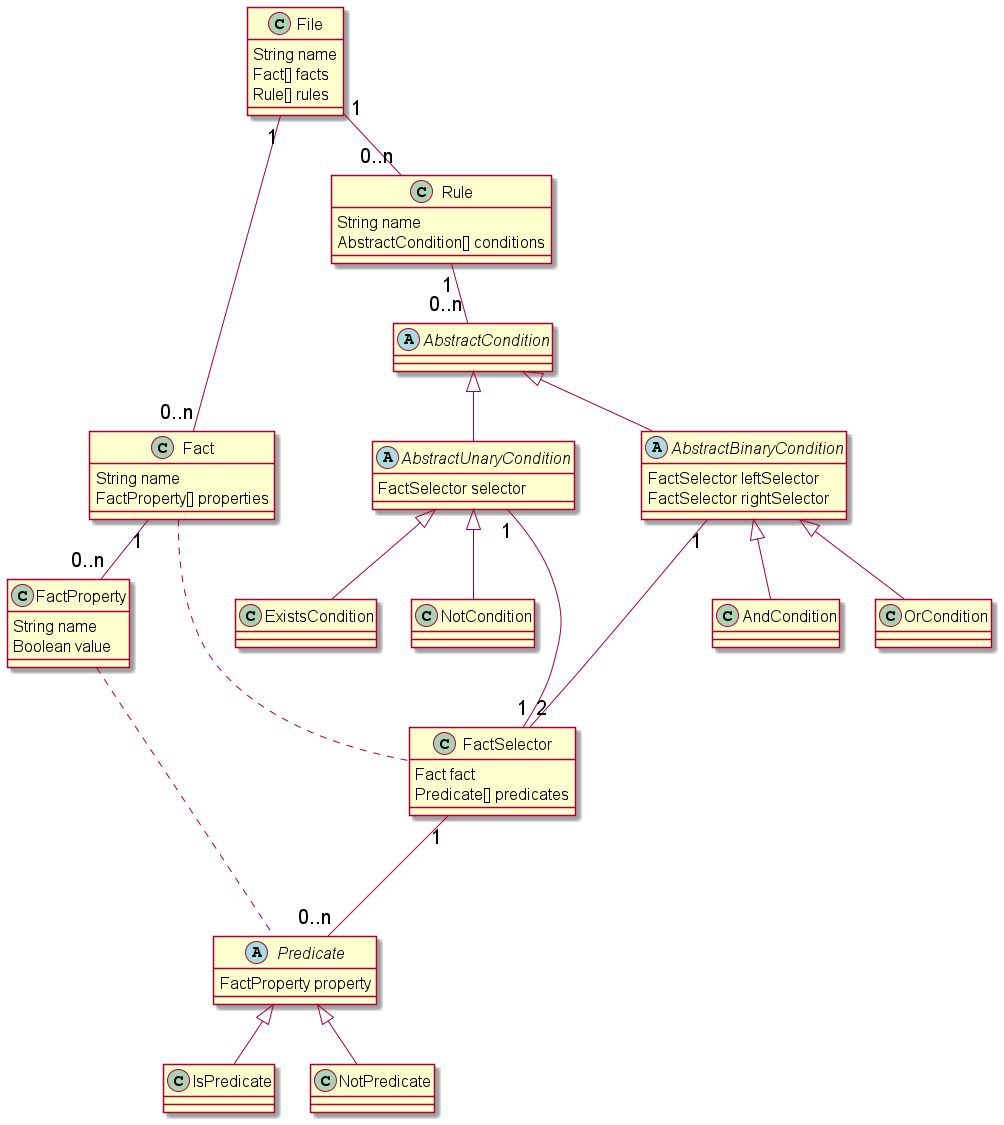
\includegraphics[width=0.95\textwidth]{Sections/images/ReallySimpleRuleLanguage3.png}}
    \caption{RSD concept hierarchy}
    \label{fig:RSDDiagram}
\end{figure}

Figure \ref{fig:RSDDiagram} shows the Concept hierarch for this straightforward implementation.

\begin{figure}
    \centering
    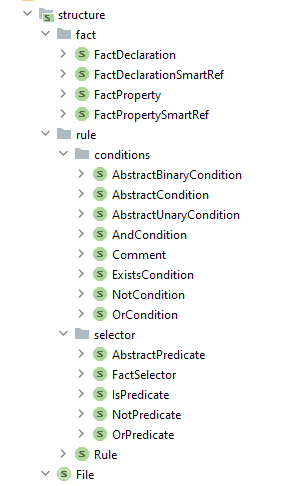
\includegraphics[width=0.9\textwidth]{Sections/images/RSRStructrure.png}
    \caption{RSD}
    \label{fig:RSDStructure}
\end{figure}

\begin{figure}
    \centering
    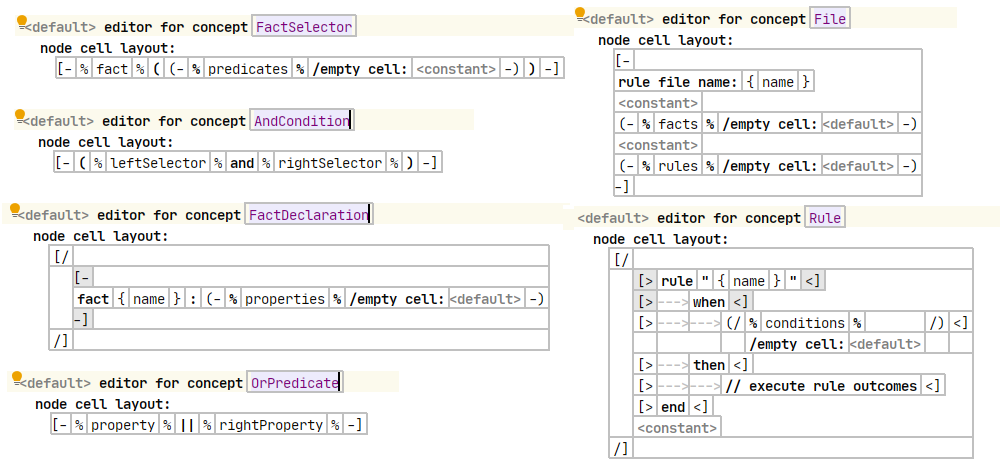
\includegraphics[width=0.9\textwidth]{Sections/images/RSREditors.png} 
    \caption{Editors}
    \label{fig:RSDEditors}
\end{figure}

We realised this design in MPS.
As the aim is to attempt different projections, we did not initially optimise for editing.
The Structure is as shown in figure \ref{fig:RSDStructure}, and the editors, including those shown in figure \ref{fig:RSDEditors}.

\begin{figure}
    \centering
    \fbox{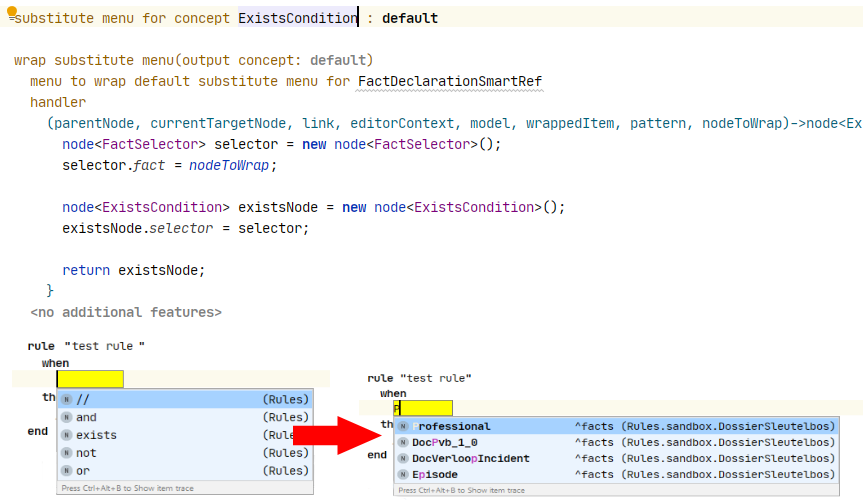
\includegraphics[width=0.95\textwidth]{Sections/images/RSRSubstituteMenu.png}} 
    \caption{RSD substitute menu}
    \label{fig:RSDSubstituteMenu}
\end{figure}

Part of our research question is using projections for reasoning about large files.
To answer this, we needed to simulate a large file.
To do this, we had to enter many \texttt{Rules}.
As this becomes tedious, we added some editing aids, including substitute menus, to speed up the entry of Conditions, as shown in figure \ref{fig:RSDSubstituteMenu}.

This image shows that we originally had to select an \texttt{ExistsCondition} Concept and select the \texttt{Fact} for the Condition.
After adding the substitute menu, we could immediately select the \texttt{Fact} we wanted, and the \texttt{ExistsCondition} would automatically wrap it with an \texttt{ExistsCondition} node.

We also added some intentions to invert incorrectly added Conditions.

\begin{figure}
    \centering
    \fbox{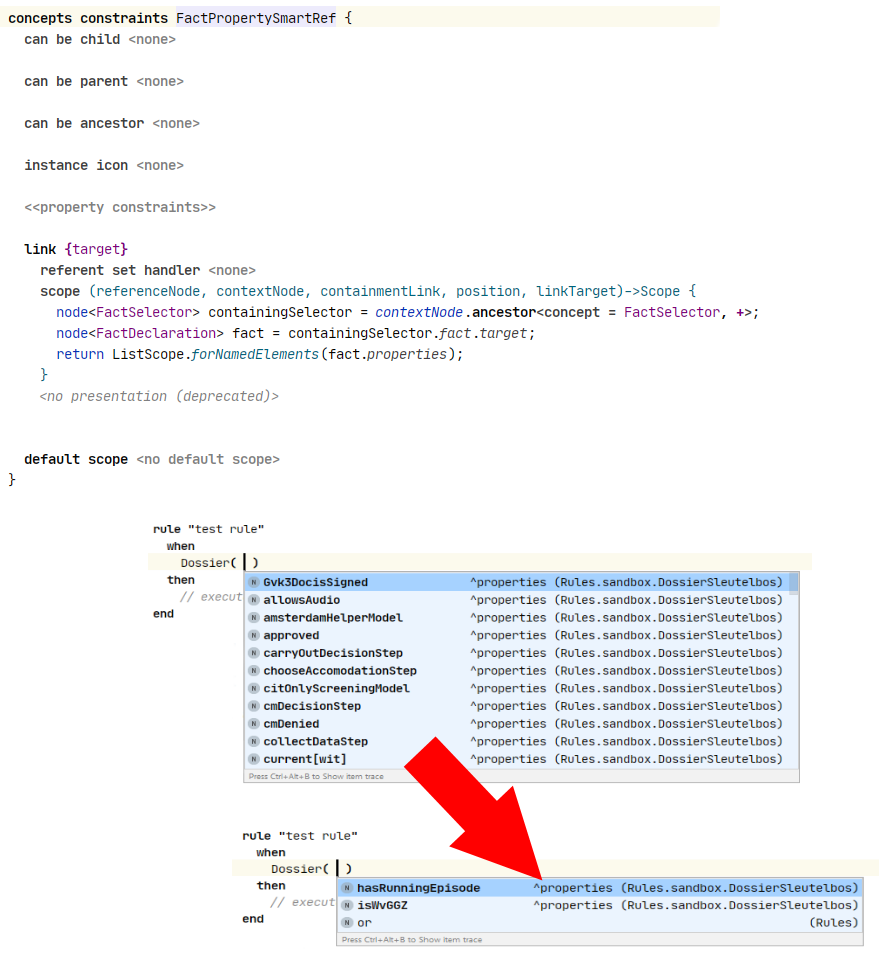
\includegraphics[width=0.95\textwidth]{Sections/images/RSRConstraint.png}}
    \caption{RSD scoping constraint}
    \label{fig:RSDConstraint}
\end{figure}

Finally, we added a Constraint to scope the \texttt{FactProperties} in \texttt{Predicates} to the \texttt{Fact} chosen in the \texttt{FactSelector}.
This scope Constraint made it much easier to select \texttt{FactProperties} in the \texttt{Predicates}, as indicated in figure \ref{fig:RSDConstraint}.

The figure shows that before adding the scoping constraint, it showed a list with dozens of potential \texttt{FactProperties}, that represented all the \texttt{FactProperties} in the model.
After adding the constraint, it only shows the two \texttt{FactProperties} associated with the \texttt{Fact} from the \texttt{FactSelector}.

Thus, we have described the entire implementation of the Really Simple Drools Language.

\begin{figure}
    \centering
    \fbox{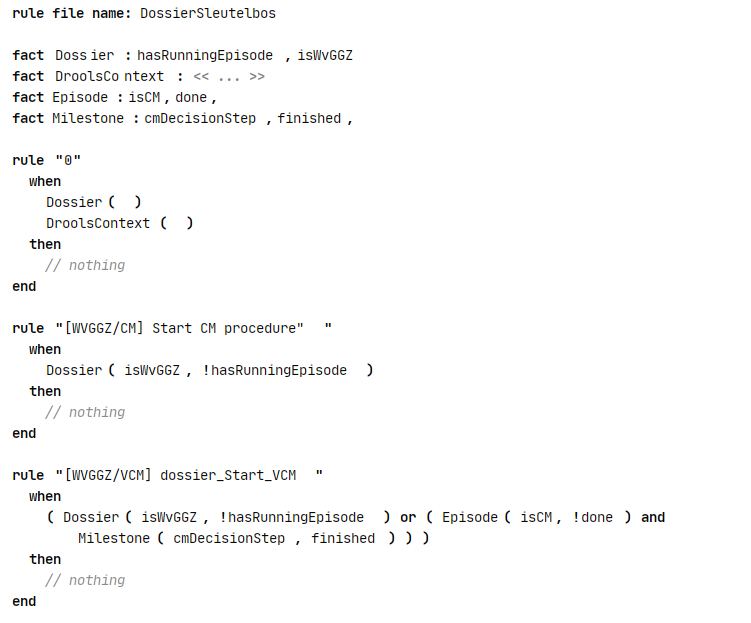
\includegraphics[width=0.95\textwidth]{Sections/images/RSRProgram.png}}
    \caption{RSD program}
    \label{fig:RSDProgram}
\end{figure}

After implementing the language, we wrote a program with many rules.
This program on which we will experiment with the different projections.
Figure \ref{fig:RSDProgram} shows an example of our default Drools-like text projection.

We discuss the alternative projections in the results section \ref{section:Results_ADR}.

\subsection{Drools-Lite Language}
\label{section:DroolsLite}

The RSD was useful as an initial language. 
However, it suffered from two significant issues.
Firstly, its limitations as a language were so substantial that it could not handle many necessary scenarios.
Secondly, our projections would be validated by developers with Drools experience, and RSD would be too alien to them.
For this reason, we needed to create a projectional language that was much closer to the Drools language.

\begin{figure}
    \centering
    \fbox{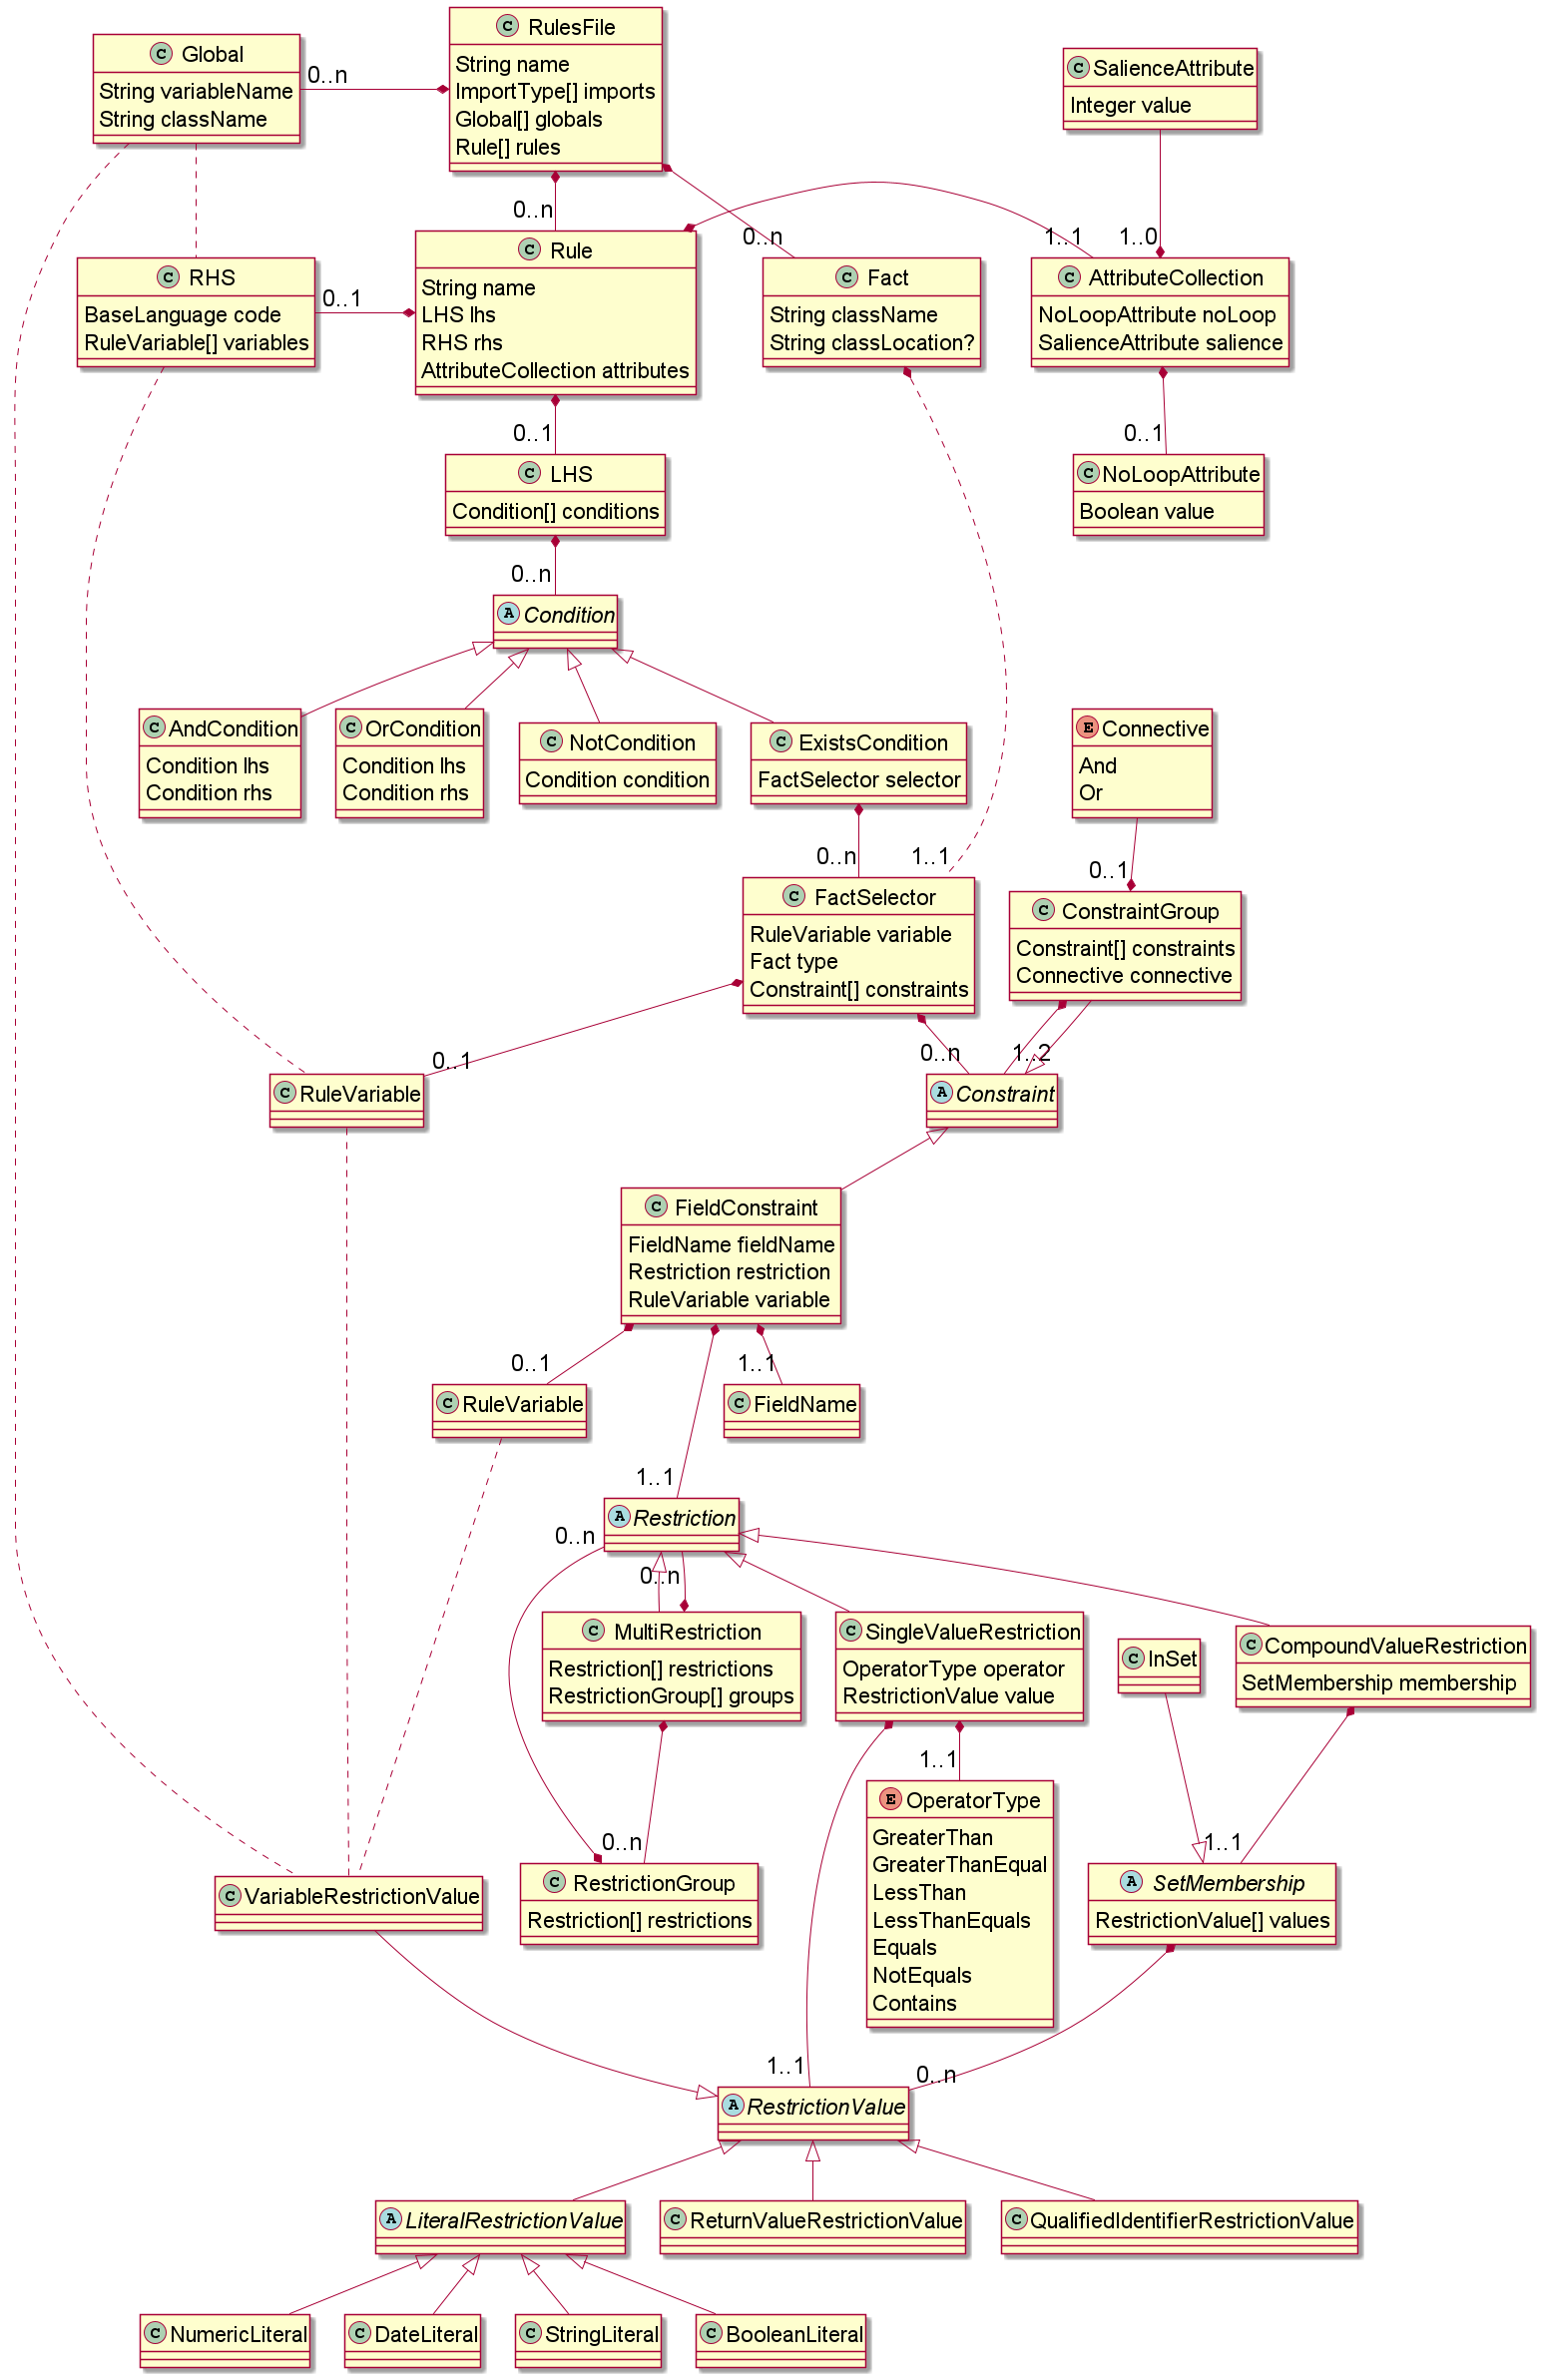
\includegraphics[width=0.90\textwidth]{Sections/images/DroolsLiteStructure.png}}
    \caption{Drools-Lite structure}
    \label{fig:DroolsLiteDiagram}
\end{figure}
 
Our following Language, Drools-Lite, contains many more of the features of Drools.
Our method of selecting the features involved implementing the examples delivered with Drools (including the corrupt politician example shown in section \ref{section:WhatIsDrools}).
We would implement just enough features to complete the examples.
Whenever we had any queries about designing Concepts, we referred to our analysis of the Drools Language, shown in appendix \ref{appendix:DroolsConceptHierarchy}.
We show the preliminary design we achieved using this method in figure \ref{fig:DroolsLiteDiagram}.
Later, there were some places we diverged a little from our design.
We merged and decoupled our Concepts when we thought it would simplify the code.

\paragraph{\texttt{RuleFile}} The \texttt{RuleFile} level statements contain \texttt{Facts}, \texttt{Globals} and \texttt{Rules}.
It also contains semantically unimportant empty lines.

\paragraph{Fact} A \texttt{Fact} has a \texttt{type} property.
We implement the \texttt{type} property using a \texttt{ClassifierType} from the MPS BaseLanguage.
This implementation allows the \texttt{RuleFile} to refer to BaseLanguage classes implemented in the same solution and from Java JAR files.

We created a smart reference Concept for this to take advantage of built-in MPS UI functionality.
A smart reference is a node with a single reference of 1:1 cardinality.
The editor builders know how to select which nodes are in scope to display to the developer if one uses this object rather than directly referencing the node it refers to.

\paragraph{FactProperty} In RSD, we had \texttt{FactProperties} as children of \texttt{Facts}.
Now that our \texttt{Facts} refer to actual classes (\texttt{ClassifierType}), our \texttt{FactProperties} should reflect this.
To do this, the Concept itself only references an \texttt{InstanceMethodDeclaration}, the MPS BaseLanguage's definition of a method signature.
We scoped the Concept to only show properties associated with a selected \texttt{Fact}.

Drools interacts with Java objects as if they are Java Beans.
To simulate this, we limited the scope of the properties to just getters, i.e., methods that start with ``get'' or ``is'', and used a Behavior to make sure they are displayed without the ``get'' or ``is'' prefix.
We also made a smart reference for this Concept.

Another option for achieving this is to have wrapped the \texttt{ClassifierType} and referenced its related \texttt{InstanceMethodDeclarations}.
We would have then had to limit the functionality of these items from the BaseLanguage.
Whilst this allows the functionality we wished for, we feel our construction offers decoupling and that, we think, correctly reflects the structure of the language.
Perhaps if we were to redo this, we would have taken the other approach.

\paragraph{\texttt{Global}} Our \texttt{Globals} are very simple.
They have a \texttt{name} and a BaseLanguage \texttt{Type}.
We added a smart reference so that \texttt{Rules} can easily use them.
The reference extended \texttt{Expression} from the BaseLanguage.
This extension is so that we could use it in the Java code of the Right-hand side.

\paragraph{\texttt{Rule}} Our \texttt{Rules} have three children: an \texttt{AttributeCollection}, a Right-hand side and a list of Conditions that make up the Left-hand side.
We created a component to describe the \texttt{Rule} editor for reuse, as we imagined that we would wrap this in other projections.

\paragraph{\texttt{RuleVariables}} The \texttt{Fact} of a \texttt{FactSelector} and the \texttt{FactProperty} of a \texttt{FieldConstraint} are bound to \texttt{RuleVariables}.
\texttt{RuleVariables} are scoped to a \texttt{Rule}.
A \texttt{RuleVariable} has only a \texttt{name} and a \texttt{type}.
We also create a smart reference for it so that it can be used elsewhere within the rule.
Like the \texttt{Global}, it extends BaseLanguage's \texttt{Expression} to be available in the Java code of the Right-hand side.

\paragraph{Right-hand side} The right-hand side of the rule, for the most part, is Java code.
To implement this, we made the right-hand side of the rule a single \texttt{StatementList}.
A \texttt{StatementList} is a list of \texttt{Statements}, both from the BaseLanguage.
We chose these because they keep track of, amongst other things, scope.

There are some non-Java, Drools specific items that are available to the right-hand side.
Items that had to be useable within the right-hand side were \texttt{Globals}, \texttt{RuleVariables} and Drools specific functions.
These all extend \texttt{Expression} from the BaseLanguage.
This extension allows seamless integration with the Java code.

The Drools specific Methods that are required are \texttt{Insert}, \texttt{InsertLogical}, \texttt{Modify}, \texttt{Delete} and \texttt{Halt}.

\begin{figure}
    \centering
    \fbox{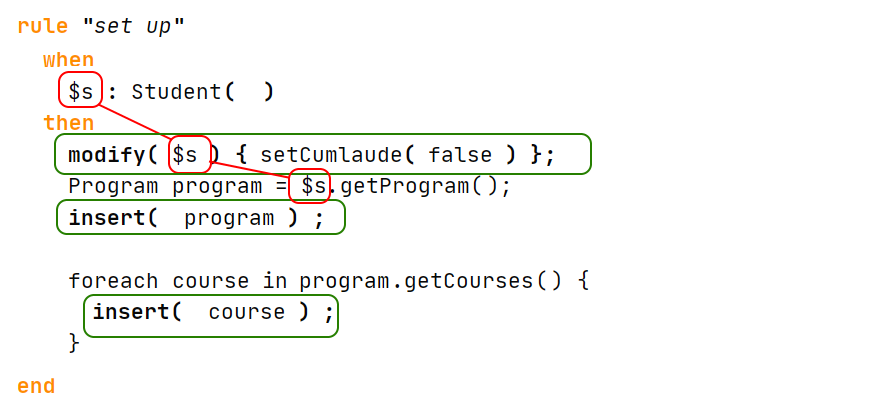
\includegraphics[width=0.70\textwidth]{Sections/images/RHS.png}}
    \caption{RHS}
    \label{fig:RHS}
\end{figure}

Figure \ref{fig:RHS} shows some of the features discussed for the right-hand side, as shown in our default projection.
The right-hand side is the text shown between the \texttt{then} keyword and the \texttt{end} keyword.
The figure shows examples of plain Java code, such as assigning to the variable \texttt{program} and the \texttt{foreach} loop.
We can also see that Drools-Lite \texttt{RuleVariable} \texttt{\$s} is in the Java statements.
We have also highlighted the Drools specific methods placed in the code, in this case \texttt{\textbf{modify}} and \texttt{\textbf{insert}}   

\begin{figure}
    \centering
    \fbox{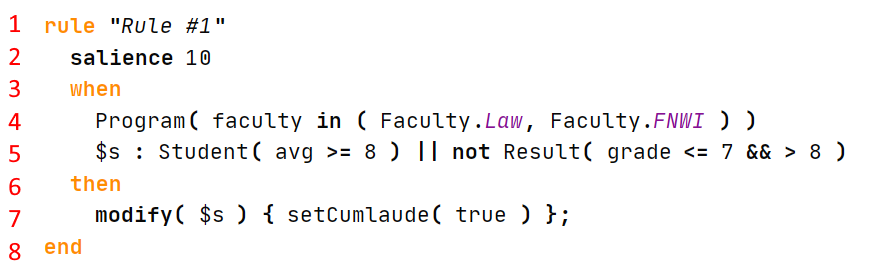
\includegraphics[width=0.85\textwidth]{Sections/images/Rule.png}}
    \caption{Rule}
    \label{fig:Rule}
\end{figure}

\paragraph{\texttt{AttributeCollection}} the \texttt{AttributeCollection} is a container to hold all the attributes that apply to a rule.
Initially, we have only implemented the \texttt{NoLoopAttribute} and \texttt{SalienceAttribute}.
A developer activates these attributes using two intentions we added to the \texttt{Rule} Concept.
On line 2 in figure \ref{fig:Rule}, we can see an example of the \texttt{SalienceAttribute} added to a rule on line 2.
\footnote{In figure \ref{fig:Rule}, we added line numbers to this figure to make it easier to talk about.
The keywords \texttt{rule} on line 1, \texttt{when} on line 3, \texttt{then} on line 6, and \texttt{end} on line 8 have no meaning in the abstract syntax.
We added them to give the developer the same look and feel as a standard Drools file.}

\paragraph{Left-hand side} This is a collection of conditions.
There are four types of conditions.
\texttt{AndCondition}, \texttt{OrCondition}, \texttt{NotCondition} and \texttt{ExistsCondition}.
\texttt{AndCondition}, \texttt{OrCondition}, and \texttt{NotCondition} have one or two children who are also conditions.
The \texttt{ExistsCondition} contains a \texttt{FactSelector}.

We added dynamic braces to only show braces around a Condition if it is a child of another Condition.
These braces add visual clarity without adding unnecessary clutter.
We also added some intentions to make it easy to switch between \texttt{ExistsCondition} and \texttt{NotCondition}.

On line 4 in figure \ref{fig:Rule}, the whole line represents an \texttt{ExistsCondition}.
Line 5 shows an \texttt{OrCondition} containing an \texttt{ExistsCondition} and a \texttt{NotCondition}.
The default editor, through an intention, can make the \texttt{ExistsCondition} explicit with an \texttt{exists} keyword.
However, the standard practice with Drools developers is to make this implicit, so this is how we show it here.

\paragraph{\texttt{FactSelector}} This always has a reference to a \texttt{Fact}.
These \texttt{Facts} are \texttt{Program} in line 4 of figure \ref{fig:Rule} and \texttt{Student} and \texttt{Result} from line 5.

Optionally, the \texttt{FactSelector} can be bound to a variable.
In figure \ref{fig:Rule}, line 5, the \texttt{FactSelector} referencing the \texttt{Student} \texttt{Fact} is bound to the \texttt{\$s} \texttt{RuleVariable}.

The \texttt{FactSelector} also contains a list of constraints on \texttt{FactProperties}, all of which must return true for the \texttt{FactSelector} to return \texttt{true}.

\paragraph{Constraints} We have three types of constraints.
\texttt{AndConstraint} and \texttt{OrConstraint} contain other constraints.
The \texttt{FieldConstraints} places restrictions on \texttt{FactProperties}.

\paragraph{FieldConstraints} A \texttt{FieldConstraint} refers to a \texttt{FactProperty} and can be bound to a variable.
It also has a restriction applied to that \texttt{FactProperty}.
Using a substitute menu, we wrapped the \texttt{FactProperty} smart reference.
This substitution automatically creates the \texttt{FieldConstraint} from the \texttt{FactProperty} selection by the developer.

There are several types of restrictions and several types of values that they can restrict.

\paragraph{\texttt{RestrictionValues}} The \texttt{RestrictionValues} that a \texttt{FactProperty} can be compared with are as follows:
\begin{itemize}    
    \setlength\itemsep{0em}
    \item \texttt{LiteralRestrictions}: These are \texttt{Integer}, \texttt{Float}, \texttt{String}, \texttt{DateTime} and \texttt{Boolean}.
    \item \texttt{VariableRestrictions}: These can be \texttt{Globals}, \texttt{RuleVariables} referring to \texttt{Facts} from the \texttt{FactSelector}, or \texttt{RuleVariables} from other \texttt{FieldConstraints}.
    \item \texttt{ReturnValue}: This compares to anything expressed as an \texttt{Expression}, which includes referring to constants or values behind qualified identifiers.
\end{itemize}

In figure \ref{fig:Rule}, on line 4, we have the return values \texttt{Faculty.Law} and \texttt{Faculty.FNWI}.
On line 5, the literal values \texttt{7} and \texttt{8}.

\paragraph{Restrictions} A \texttt{SingleValueRestriction} compares a \texttt{FactProperty} against a value.
A \texttt{MultiRestriction} compares a \texttt{FactProperty} against multiple values, not necessarily using the same comparison for each value.
A \texttt{SetMembership} restriction checks if a \texttt{FactProperty} is a member or not a member of a group.

In figure \ref{fig:Rule} on line 4 a \texttt{SetMembership} restriction is shown with the \texttt{in ( Faculty.Law, Faculty.FNWI )} text.
Line 5 in the first \texttt{FactSelector} there is the \texttt{SingleValue} restriction \texttt{ avg >= 8}.
The second \texttt{FactSelector} shows a \texttt{MultiRestrictions} \texttt{grade <= 7 \&\& > 8}.

Thus, we have described the pertinent implementation details of the Drools-Lite language.

\subsection{Wireframes}

There are some potential projections we have conceived for which there is not sufficient time to implement.
We want Drools experts to assess these and thus would like them to appear as realistic as possible to the assessors.

Our solution to this conundrum is to develop these presentations in a wireframing tool.
The wireframe tool we chose was Axure\cite{Axure_ProductPage}.
We chose this because we had previous experience with the product.
Also, it is available to students for free.

We settled on two possible projectional programming aids: Truth table and circuit diagram.
We will discuss these in more detail in the results section.
